% !TEX program = pdflatex
% ============================================================================
% WINE 2026 submission (double-blind, anonymized). Self-contained single file;
% all figures TikZ/pgfplots (no external images), compiles standalone.
% Formal results are keyed by superscripts L1..L13 to the appendix table;
% full statements and proof artifacts available from the authors on request.
% ============================================================================

\documentclass[runningheads]{llncs}

\usepackage[utf8]{inputenc}
\usepackage[T1]{fontenc}
\usepackage{amsmath,amssymb}
\usepackage{mathtools}
\usepackage{booktabs}
\usepackage{tabularx}
\usepackage{enumitem}
\usepackage{xcolor}
\usepackage{tikz}
\usepackage{pgfplots}
\pgfplotsset{compat=1.17}
\usetikzlibrary{arrows.meta,calc,decorations.pathreplacing}
\usepackage{hyperref}
\hypersetup{colorlinks=true,linkcolor=black,citecolor=black,urlcolor=blue}
\usepackage[expansion=false]{microtype}
\emergencystretch=3em

% A consistent provenance macro for every Lean citation: verified in Lean by
% Harmonic's Aristotle prover (compiled server-side; not re-run locally).
\newcommand{\tfp}{\emph{verified in Lean}}

\title{A Single Dynamic AMM Pricing American-Style Perpetual Options
Across the Strike Continuum}
\titlerunning{A Single Dynamic AMM for American-Style Perpetual Options}

\author{}
\authorrunning{Anonymous submission to WINE 2026}
\institute{}

\begin{document}
\maketitle

% ===========================================================================
\begin{abstract}
American-style perpetual options let perpetual-futures traders reduce
liquidation risk without closing the position. We show that a \emph{single}
liquidity pool prices that protection at every strike at once. The pool runs on
the weighted constant-product (``Balancer'') curve, with one structural change:
a trade does not slide a point along the curve but \emph{skews} the curve
instead. The stored skew is the pricing state: from one pool state we read
every out-of-the-money call and put in closed form, with an exact
\emph{American} early-exercise level and a smooth join between waiting and
exercising. One knob, set from the asset's volatility, fixes the whole
book's steepness. The core results are verified in Lean (by Harmonic's
Aristotle prover).

\keywords{Automated market maker \and Decentralized finance \and Perpetual
options \and Optimal stopping \and Smooth pasting \and Formal verification}
\end{abstract}

% ===========================================================================
\section{Introduction and contributions}\label{sec:idea}
% ===========================================================================

In the pool's reserve plane, every strike is a \emph{ray} from the origin. A
trade executes where its ray meets the pool curve, and it \emph{skews the
curve} at that point: the weight of the Balancer invariant is updated per
trade, so the pool carries its trading history as a stored skew.

That stored skew is the pricing state, and the division of labour is strict
throughout: \emph{the pool only bookkeeps}---it stores the state $(x,y,w)$,
updates it per trade, and prices slippage---while \emph{every economic
quantity is the option-pricing layer} reading that state. From the single
state the mechanism reads the value of \emph{every} out-of-the-money call and
put in closed form---no premium object, no expiry, no per-strike order
book---with an exact American early-exercise boundary, one volatility knob for
the whole book, and a Lean-verified core. The conditions are stated plainly
throughout: what is verified in Lean, what is an engine measurement, and where
solvency stays conditional.

\paragraph{Contributions.}
The curve family itself is \emph{not} new: each trade's arc is, after a change of
coordinates, an ordinary constant product (Section~\ref{sec:warp})---a translated
market maker in the sense of Evans~\cite{evans2020} and the replication theory of
Angeris--Evans--Chitra~\cite{angeris-replicating}. What is new is:
\begin{enumerate}[leftmargin=2em,itemsep=2pt]
  \item a \emph{per-trade weight update} that turns a Balancer pool into a
        state machine whose stored skew prices a tradable claim at every strike
        (Section~\ref{sec:warp});
  \item a \emph{semantic layer} over that pool---strike-as-a-ray, the mark, and
        settlement---that reads a continuum of option values from one pool state
        (Section~\ref{sec:continuum}; settlement in Appendix~\ref{app:properties});
  \item an \emph{exact American exercise rule}: a closed-form early-exercise
        boundary $S^{\ast}=K\,m\gamma/(m\gamma+1)$ (put form; calls mirror),
        where the exercised
        payoff line joins the waiting-value curve \emph{tangentially}---same
        value, same slope, no kink (``smooth pasting'') (base form
        $K\gamma/(\gamma+1)$ at $m=1$; $K$ the dollar strike, $\gamma>1$ the
        curve's convexity exponent, $m$ the knob below), with a smooth
        value-and-slope join and no new parameters, tied to the classical
        perpetual-American (Merton) problem (Section~\ref{sec:american});
  \item a single \emph{volatility-calibrated} steepness knob $m$ that sets
        the option-value steepness uniformly across strikes---trades never
        move it (Section~\ref{sec:lens});
\end{enumerate}
together with an honest formal-verification ledger (Appendix~\ref{sec:frontier})
stating exactly what is verified in Lean, under what label, and where the open
frontier is---solvency is conditional on a funding port shown necessary but not
discharged. The object throughout is the mechanism itself---the pool \emph{is} the
option market; equilibrium and welfare analysis are future work
(Section~\ref{sec:limits}).

% ===========================================================================
\section{The AMM construction}\label{sec:warp}
% ===========================================================================

\begin{figure}[t]
\centering
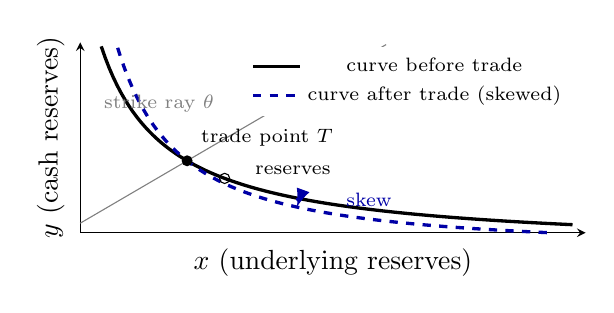
\begin{tikzpicture}[scale=1.0,>=Latex]
  \begin{axis}[
      width=8.0cm, height=4.0cm,
      xlabel={$x$ (underlying reserves)}, ylabel={$y$ (cash reserves)},
      xmin=0.35, xmax=4.2, ymin=0.35, ymax=4.2,
      xtick=\empty, ytick=\empty,
      axis lines=left, clip=false, samples=120,
      legend style={at={(0.98,0.98)},anchor=north east,font=\scriptsize,draw=none}]
    % Balancer level curves (illustrative): y = k^{1/(1-w)} x^{-w/(1-w)}.
    % base curve w=1/2: y = c/x  with c=2.1
    \addplot[very thick,domain=0.51:4.1,black] {2.1/x};
    \addlegendentry{curve before trade}
    % skewed curve: a GENUINE power law c'/x^p (p=1.35, no additive offset),
    % chosen to pass through the trade point T; domain starts at 0.635 so the
    % curve stays inside the frame (hits y=4.1 at x=0.635).
    \addplot[very thick,dashed,domain=0.635:3.92,blue!65!black] {2.2146/x^(1.35)};
    \addlegendentry{curve after trade (skewed)}
    % strike ray from origin: y = theta x with theta=1.55
    \addplot[gray,thin,domain=0.35:2.68] {1.55*x};
    \node[gray,font=\scriptsize] at (axis cs:0.95,2.95) {strike ray $\theta$};
    % trade point T: ray meets BOTH curves at (1.164,1.804). The trade skews
    % the curve AT T, so before- and after-curve cross here. (2.1/1.164=1.804;
    % 2.2146/1.164^1.35=1.804; 1.55*1.164=1.804.)
    \node[circle,fill=black,inner sep=1.4pt,label={[font=\scriptsize]above right:trade point $T$}]
      at (axis cs:1.164,1.804) {};
    % skew arrow: at a fixed x=2.0 out on the wing, base y=1.05 moves down to
    % after y=0.869 -- the skew of the wing past T.
    \draw[->,thick,blue!65!black] (axis cs:2.0,1.05) to[bend left=20] (axis cs:2.0,0.869);
    \node[blue!65!black,font=\scriptsize] at (axis cs:2.55,1.02) {skew};
    % reserves point on the base curve for contrast (2.1/1.45=1.448)
    \node[circle,draw=black,inner sep=1.3pt] at (axis cs:1.45,1.448) {};
    \node[font=\scriptsize] at (axis cs:1.97,1.62) {reserves};
  \end{axis}
\end{tikzpicture}
\caption{A trade occurs where a \emph{strike ray} $\theta$ meets the curve (point
$T$) and \emph{skews} the curve there rather than sliding the reserve point.
Both curves pass through $T$; the skewed wing (dashed) is a genuine power law
$c'/x^{p}$, same constant-product family as the base $c/x$. The stored skew is the
pricing state: every strike's option value is read from it. Curves illustrative.}
\label{fig:warp}
\end{figure}

\subsection{The Balancer curve}
We work on the two-asset slice of Balancer's weighted constant-product family,
in the plane of reserves $x$ (underlying) and $y$ (cash):
\begin{equation}
  x^{w}\,y^{1-w}=k ,
  \label{eq:balancer}
\end{equation}
a fixed weighted geometric mean of the reserves. The \emph{weight} $w\in(0,1)$
says how the curve \emph{skews} between the assets---$w=\tfrac12$ is symmetric,
and pushing $w$ off $\tfrac12$ skews pricing toward one asset; the \emph{level}
$k$ is its overall scale. In ordinary use $w$ and $k$ are fixed and trades slide
$(x,y)$ along the curve.

\subsection{Trades skew the curve}
Our one structural change: \emph{a trade updates the weight $w$}, and a change in
$w$ skews the curve~\eqref{eq:balancer}. The pool becomes a
\emph{state-transition system}, one state update per trade. The stored state is
the triple $(x,y,w)$, with $w$ genuine memory; the level $k=x^{w}y^{1-w}$ is a
dependent \emph{readout} that trades do not hold constant.

Two views of a trade coincide. Sliding the origin to \emph{shifted virtual
reserves} $u=x-\alpha$ and $v=y-\beta$, where $\alpha=xw$ and $\beta=y(1-w)$ are
curve offsets, each trade's arc satisfies the ordinary constant product
$u\,v=\text{const}$: a \emph{translated} constant-function market maker in the
sense of Evans~\cite{evans2020}, so the ``skewing'' picture is a re-description of
a weight change, not a new invariant. \textbf{This is exactly why we do not claim
the curve family as a contribution}---we claim the per-trade weight \emph{update}
and the semantic layer built on it.

\subsection{Trades happen anywhere on the curve}
In ordinary market makers a trade is always at the reserve point; here it may land
at \emph{any} out-of-the-money point. Each ray from the origin---a line
$y=\theta x$ of fixed reserve ratio---is identified with one strike. The ray meets
the curve at a single \emph{trade point}, and a transaction there is handled as if
that point were the reserve point: the conservation law is applied locally, at the
trade's own point. The $\theta=1$ ray is the at-the-money strike; steeper and
shallower rays split the continuum into the call and put \emph{wings}, both priced
from the same $(x,y,w)$ state (Figure~\ref{fig:warp}).

Explicitly, write $T=(x_{T},y_{T})$ for the trade point on the ray, and
$\alpha_{T}=x_{T}\,w$, $\beta_{T}=y_{T}\,(1-w)$ for the curve offsets of
Section~\ref{sec:warp} evaluated \emph{at $T$}. A trade whose cash leg is
$\Delta y$ (the cash the trader pays in or takes out) updates the state
$(x,y,w)$ by
% --- VERIFICATION of eq:tradeupdate against the arithmetic exhibit below ---
% From (x,y,w)=(10,10,1/2): curve x^{1/2}y^{1/2}=10, i.e. xy=100; the ray
% theta=4 meets it at T=(5,20). alpha_T=5*(1/2)=5/2, beta_T=20*(1/2)=10.
% Delta y = 1:
%   Delta x = -(5/2)(10)(1)/((20-10)(20+1-10)) = -25/110 = -5/22,
%   w' = alpha_T/(x_T+Delta x) = (5/2)/(5-5/22) = (5/2)/(105/22) = 55/105
%      = 11/21.   [matches the exhibit's w' = 11/21]
% The naive global recompute alpha/x' = 5/(10-5/22) = 110/215 = 22/43
% [matches the exhibit's 22/43]. Equivalent increment form (American draft
% eq:trade): Delta w = beta_T*Delta y/(y_T(y_T+Delta y)) = 10/(20*21) = 1/42;
% 1/2 + 1/42 = 11/21. Same closed form as the engine's tradeUpdate
% (HEAD v28, engine lines ~1689-97): dx = -alpha*beta*dy/((y-beta)(y+dy-beta)),
% with alpha,beta preserved; identity w' = alpha_T/(x_T+Dx) = w + Dw checked
% exactly (rational arithmetic) on random states.
\begin{equation}
  y'=y+\Delta y,\qquad
  x'=x+\Delta x,\quad
  \Delta x=-\frac{\alpha_{T}\,\beta_{T}\,\Delta y}
                 {(y_{T}-\beta_{T})\,(y_{T}+\Delta y-\beta_{T})},\qquad
  w'=\frac{\alpha_{T}}{x_{T}+\Delta x},
  \label{eq:tradeupdate}
\end{equation}
on the admissible domain $y_{T}+\Delta y>\beta_{T}$ and subject to reserve
feasibility ($x+\Delta x>0$, $y+\Delta y>0$). In words: the flows
$\Delta x,\Delta y$ are the translated-constant-product amounts computed at the
trade's own point $T$ rather than at the reserve point (conserving the local pair
$\alpha_{T},\beta_{T}$), drawn from the pool's actual reserves $(x,y)$; the new
skew $w'$ is read off at the displaced trade point $x_{T}+\Delta x$.

A spot swap is the special case where the trade point \emph{is} the reserve
point, and only there does the trade trace the familiar constant-product
trajectory.
Off-the-money trades genuinely change the global offsets $\alpha,\beta$ by design;
those were never claimed constant across such trades. That $w$ must be stored
(rather than recomputed from $x$) is shown by an arithmetic exhibit
of~\eqref{eq:tradeupdate}: from $(x,y,w)=(10,10,\tfrac12)$ the $\theta=4$ trade
point is $T=(5,20)$, and a unit cash leg $\Delta y=1$ gives $\Delta x=-5/22$ and
$w'=11/21$---not the global recompute $\alpha/x'=22/43$ (pre-trade $\alpha=xw$
over the new reserve $x'$). The pool invariant, the trade
law~\eqref{eq:tradeupdate}, and the trade/rebase commutation are verified in
Lean\textsuperscript{L1,L2} (Appendix~\ref{app:lean}).

\paragraph{Division of labour.}
The pool is the \emph{bookkeeping} layer and nothing more: it stores the
state $(x,y,w)$, updates it per trade by~\eqref{eq:tradeupdate}, and---because
each read walks the live curve---prices \emph{slippage}. Every economic
quantity is set by the \emph{option-pricing} layer of
Section~\ref{sec:continuum} reading that state: position values, trade
sizing, payouts. The pool never holds premium and is never a counterparty
(Section~\ref{sec:exec}).


% ===========================================================================
\section{How a trade runs}\label{sec:exec}
% ===========================================================================
The life of a position, in the order a trader lives it. Throughout, remember
the division of labour: the \emph{pricing layer} decides every economic
number; the \emph{pool} only bookkeeps the flows and charges the slippage.
These are specification-level statements of the shipped design, not
Lean-verified results.
\begin{enumerate}[leftmargin=2em,itemsep=1pt]
  \item \textbf{You open.} You hold a perpetual future and pick a strike. A
    slice of your perp is \emph{carved}---its notional, equity, and entry
    mark frozen as your escrow. Your position is a \emph{band}: two option
    legs on opposite wings, one sold and one bought. The sold leg is valued
    by the pricing layer, and the bought leg's size (notional) is that value
    divided by the bought leg's per-unit price:
    $N_{\mathrm{buy}}=V_{\mathrm{sell}}/v_{\mathrm{buy}}$, an option-price
    \emph{ratio}. Premium never touches the pool; slippage enters because the
    second leg is priced on the pool as the first leg left it. A small fee
    ($0.01\%$ of notional) is paid from your side's \emph{club}---its pooled
    equity, your counterparty in step~5---never into the pool.
  \item \textbf{The pool bookkeeps your open.} In the pool's books an
    option is just an asset swap \emph{at a strike}: buying a call is booked
    as buying the underlying at the strike, buying a put as selling the
    underlying at the strike---and selling either leg is the reverse. So each
    leg moves the pool by $\Delta y=\pm N\,K_{\mathrm{tx}}$: notional times
    the strike, in dollars. The booking strike is \emph{your} strike passed
    through the lens---equal to your chosen strike at $m=1$, pushed further
    out along the curve as $m$ grows
    ($\theta_{\mathrm{tx}}=\mathrm{mode}\cdot(\mathrm{chosen}/\mathrm{mode})^{m}$,
    the mode being the at-the-money ray; Section~\ref{sec:lens})---and its
    dollar value $K_{\mathrm{tx}}$ is frozen at open. If your cash
    leg exceeds the pool's usable depth, the trade is rejected outright with
    the numbers---never silently capped.
  \item \textbf{You hold.} Funding is metered by the same-slope funding read of
    Section~\ref{sec:funding}; the curve's steepness $\gamma=w/(1-w)$ is
    read \emph{live} at every step (it moves as trades skew the curve; the
    knob $m$ is never moved by trades).
  \item \textbf{You close.} Settlement is at the strike \emph{you chose}.
    Each leg still on the pool reverses its opening swap at the \emph{same}
    frozen $K_{\mathrm{tx}}$---the reserves round-trip exactly. A leg past
    its boundary has left the pool's world: it settles to cash at its mark,
    no pool swap (the two-case rule of Appendix~\ref{sec:settlement}).
  \item \textbf{You get paid.} Your legs net in perp units; the net converts
    to cash at your carved slice's closing equity, scaled by $L_{0}$ (the
    product's leverage factor, frozen at open):
    payout $=L_{0}\times(\text{net result})\times(\text{carved equity})$.
    The counterparty is your club (step~1); a drained club pays
    nothing---positive payouts stop at zero club equity.
\end{enumerate}
One background mechanic: liquidity provision resizes the pool
\emph{isotropically}---price and skew untouched; it is not a trade.


% ===========================================================================
\section{Options across the strike continuum}\label{sec:continuum}
% ===========================================================================

\subsection{The perpetual option}
A perpetual option is a never-expiring claim on favourable price action---upward
for a call, downward for a put---past a strike $K$. Composed with a perpetual
future, it caps the trader's loss beyond $K$ without forcing the position closed;
the only decision the holder faces is \emph{when} to realise it.

\subsection{The mark: one ray, one curve}
The worth of a position is its \emph{mark}, and the mark is one geometric
read: the strike's ray meets the \emph{pool curve} at one point, and the value
is read off at that meet. One ray, one curve---no second object. (A comparison
across \emph{two} curves appears exactly once in this paper, in funding:
the same slope located on the pool curve and on the anchor curve,
Section~\ref{sec:funding}.) In dollars the meet sits at moneyness $S/K$ (spot
over strike), and the map from the meet to the option price is explicit---a
power law, welded to the exercised payoff (put wing shown; the call wing
mirrors it by reflection, Section~\ref{app:properties}):
\begin{equation}
  \mathrm{mark}(\theta)\;=\;
  \begin{cases}
    \dfrac{1}{g+1}\Bigl(\dfrac{S^{\ast}}{S}\Bigr)^{g}, & S\ge S^{\ast}
      \quad\text{(waiting: a power of the ray read)},\\[6pt]
    1-\dfrac{S}{K}, & S<S^{\ast}\quad\text{(exercised: parity)},
  \end{cases}
  \label{eq:mark}
\end{equation}
with $g=m\gamma$ the lensed steepness ($\gamma$ the curve's own steepness,
read from the skew; $m$ the vol knob---both Section~\ref{sec:lens}) and
$S^{\ast}=K\,g/(g+1)$ the free boundary solved in
Section~\ref{sec:american}. One ray, one curve, one power law. The mark is
denominated as a fraction of the wing's \emph{escrow unit} (one full perpetual
future): a position of notional $q$ is worth $q\cdot\mathrm{mark}$, and
nothing else---no separate premium object, no expiry, no intrinsic/extrinsic
split; the whole continuum is priced from the one pool state $(x,y,w)$. The
mark reaches $1$ only at \emph{full} exercise; at the money it is the waiting
value ($0.148$ at $g=2$, Appendix~\ref{app:spec}), not $1$.
Figure~\ref{fig:read} draws the whole map, including how the lens of
Section~\ref{sec:lens} enters both the read and the transaction.

\begin{figure}[t]
\centering
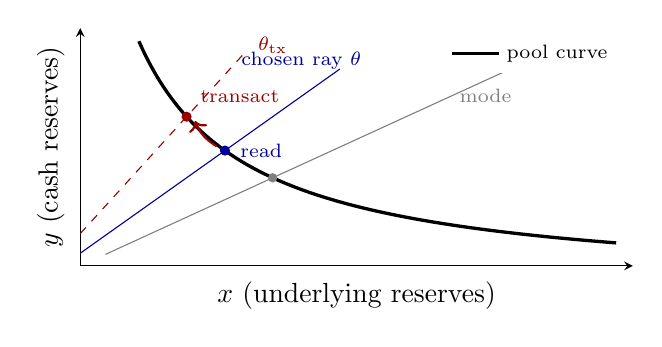
\begin{tikzpicture}
  \begin{axis}[
      width=8.6cm, height=4.6cm,
      xlabel={$x$ (underlying reserves)}, ylabel={$y$ (cash reserves)},
      xmin=0.3, xmax=3.6, ymin=0.3, ymax=3.4,
      xtick=\empty, ytick=\empty,
      axis lines=left, clip=false, samples=120,
      legend style={at={(0.98,0.98)},anchor=north east,font=\scriptsize,draw=none}]
    % pool curve y=2.1/x
    \addplot[very thick,black,domain=0.65:3.5] {2.1/x};
    \addlegendentry{pool curve}
    % mode ray y=x (ATM): meets curve at (1.449,1.449)
    \addplot[gray,thin,domain=0.45:2.9] {x};
    \node[gray,font=\scriptsize] at (axis cs:2.72,2.52) {mode};
    % chosen strike ray y=1.55x: meets curve at (1.164,1.804)
    \addplot[blue!60!black,thin,domain=0.3:1.85] {1.55*x};
    \node[blue!60!black,font=\scriptsize] at (axis cs:1.62,2.98) {chosen ray $\theta$};
    % lens tx ray m=2: theta_tx=1.55^2=2.4025: meets curve at (0.935,2.246)
    \addplot[red!60!black,dashed,thin,domain=0.3:1.28] {2.4025*x};
    \node[red!60!black,font=\scriptsize] at (axis cs:1.45,3.18) {$\theta_{\mathrm{tx}}$};
    % intersection points
    \node[circle,fill=blue!60!black,inner sep=1.3pt,
      label={[font=\scriptsize,blue!60!black]right:read}] at (axis cs:1.164,1.804) {};
    \node[circle,fill=red!60!black,inner sep=1.3pt,
      label={[font=\scriptsize,red!60!black]above right:transact}] at (axis cs:0.935,2.246) {};
    \node[circle,fill=gray,inner sep=1.2pt] at (axis cs:1.449,1.449) {};
    \draw[->,thick,red!60!black] (axis cs:1.115,1.86) to[bend left=18] (axis cs:0.985,2.19);
  \end{axis}
\end{tikzpicture}
\caption{From strike ray to option price, through the lens. A strike is a ray;
its meet with the pool curve is where everything happens. \emph{Reading}: the
meet sits at moneyness $S/K$, and the mark is the power law of
Eq.~\eqref{eq:mark} with lensed exponent $g=m\gamma$. \emph{Transacting}: the
swap executes further out, on the lens ray
$\theta_{\mathrm{tx}}=\mathrm{mode}\cdot(\theta/\mathrm{mode})^{m}$ (the
\emph{mode} is the pool's at-the-money ray; drawn for $m=2$), frozen at open. One knob $m$ steepens the read and displaces the
transaction in the same direction.}
\label{fig:read}
\end{figure}

\subsection{Rebasing: the frame tracks the market}
The pool follows the outside (oracle) price by \emph{rebasing}: on each oracle
update the whole picture---curve and every strike ray together---is rescaled by
one factor $r>0$ ($x\to rx$, $\alpha\to r\alpha$, $k\to r^{w}k$, each ray
$\theta\to\theta/r$), so the pool's centre tracks the market while no
position gains or loses (a rebase is a change of coordinates, not a trade).
Internally the frame is anchored by a reference price $P=N_{y}/N_{x}$ (the
\emph{carry}, the ratio of the pool's notional cash to notional underlying
holdings); a strike is registered by its log-distance
$u=\log(\text{price})-\log P$. Trades and rebases \emph{commute}, so the
pricing frame is well defined regardless of their order
(\tfp{}\textsuperscript{L2}); the full transform and its implications are in
Appendix~\ref{app:spec}.

\subsection{Funding}\label{sec:funding}
Mirroring a perpetual future, a position accrues \emph{funding} at a rate
proportional to how far the live curve deviates from the symmetric
($w=\tfrac12$) \emph{anchor} curve, read \emph{like slope to like slope}:
the slope at the position's strike is located on \emph{both} curves, and the
deviation is the gap between the two ray angles at which they attain it
(Figure~\ref{fig:funding}), through the vol knob of Section~\ref{sec:lens}.
Matching the slope---rather than the ray---is what respects the at-the-money
point: on-anchor, both curves attain the reference slope at the same ray, so
the deviation---and the rate---vanishes exactly there. The crowded side pays the contrarian side; on-anchor
the rate is exactly zero; a rebase bounds how fast drift accumulates into the
deviation. This paper fixes the \emph{rate} law (the exact shipped form is in
Appendix~\ref{app:spec}); the cash-transfer routing is implementation-level
and we do not claim the rate neutralises any specific equilibrium drift---both
deferred (Appendix~\ref{sec:frontier}).

\begin{figure}[t]
\centering
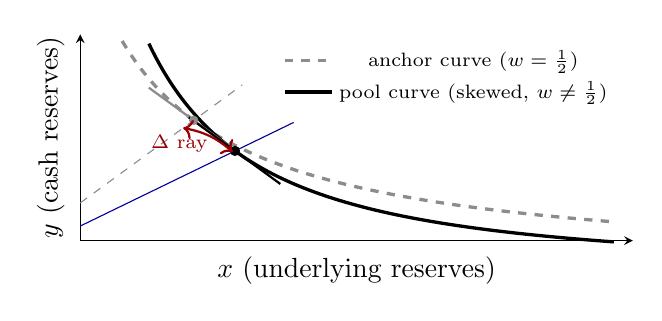
\begin{tikzpicture}
  \begin{axis}[
      width=8.6cm, height=4.2cm,
      xlabel={$x$ (underlying reserves)}, ylabel={$y$ (cash reserves)},
      xmin=0.5, xmax=3.4, ymin=0.4, ymax=3.0,
      xtick=\empty, ytick=\empty,
      axis lines=left, clip=false, samples=140,
      legend style={at={(0.98,0.98)},anchor=north east,font=\scriptsize,draw=none}]
    % anchor curve w=1/2: y=2.1/x ; skewed pool curve w=0.6: y=2.3004/x^1.5.
    % SAME SLOPE s=1.75 located on both (entry 386): anchor attains it at
    % (1.0954,1.9170) [ray 1.75], pool at (1.3120,1.5307) [ray 1.1667].
    \addplot[very thick,black!45,dashed,domain=0.72:3.3] {2.1/x};
    \addlegendentry{anchor curve ($w=\tfrac12$)}
    \addplot[very thick,black,domain=0.86:3.3] {2.3004/x^(1.5)};
    \addlegendentry{pool curve (skewed, $w\neq\tfrac12$)}
    % the two rays at which each curve attains the SAME slope
    \addplot[black!45,thin,dashed,domain=0.5:1.35] {1.75*x};
    \addplot[blue!60!black,thin,domain=0.5:1.62] {1.1667*x};
    % parallel tangent segments, both slope -1.75
    \draw[black!45,thick]
      (axis cs:0.86,{1.9170+1.75*0.235}) -- (axis cs:1.33,{1.9170-1.75*0.235});
    \draw[black,thick]
      (axis cs:1.07,{1.5307+1.75*0.242}) -- (axis cs:1.55,{1.5307-1.75*0.238});
    \node[circle,fill=black!45,inner sep=1.2pt] at (axis cs:1.0954,1.9170) {};
    \node[circle,fill=black,inner sep=1.3pt] at (axis cs:1.3120,1.5307) {};
    \draw[<->,red!60!black,thick] (axis cs:1.04,1.82) to[bend left=15] (axis cs:1.30,1.5167);
    \node[red!60!black,font=\scriptsize] at (axis cs:1.02,1.62) {$\Delta$ ray};
  \end{axis}
\end{tikzpicture}
\caption{The funding read: the \emph{same slope} is located on both
curves---the live (skewed) pool curve and the $w=\tfrac12$ anchor---and the
funding rate is proportional to the gap between the two ray angles at which
they attain it ($\Delta$~ray; the parallel segments are the two equal-slope
tangents, drawn for slope $1.75$: rays $1.75$ vs $1.167$). Matching slope
rather than ray is what respects the at-the-money point: on-anchor both
curves attain the reference slope at the same ray, so the deviation---and
the rate---is exactly zero. Exact rate law: Appendix~\ref{app:spec}.}
\label{fig:funding}
\end{figure}

% ===========================================================================
\section{The vol knob (the lens)}\label{sec:lens}
% ===========================================================================

\begin{figure}[t]
\centering
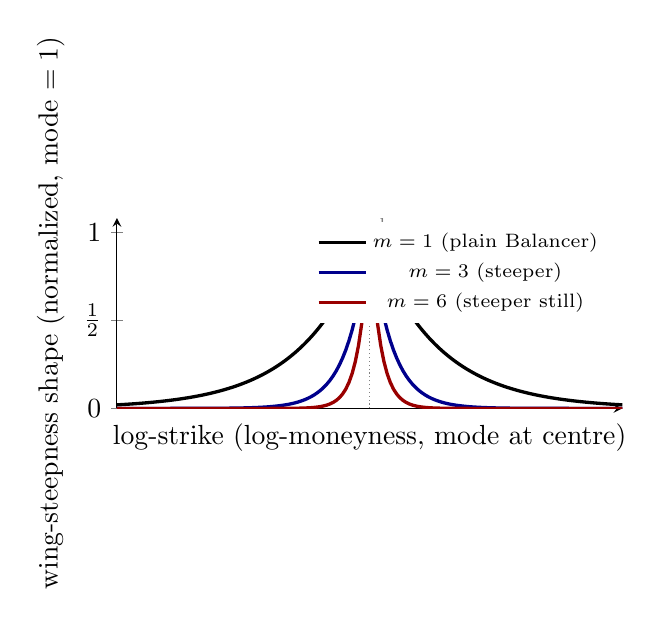
\begin{tikzpicture}
  \begin{axis}[
      width=8.0cm, height=4.0cm,
      xlabel={log-strike (log-moneyness, mode at centre)},
      ylabel={wing-steepness shape (normalized, mode $=1$)},
      xmin=-2.6, xmax=2.6, ymin=0, ymax=1.08,
      xtick=\empty, ytick={0,0.5,1}, yticklabels={$0$,$\tfrac12$,$1$},
      axis lines=left, samples=160,
      legend style={at={(0.98,0.98)},anchor=north east,font=\scriptsize,draw=none}]
    % normalized steepness shape (mode/theta)^{m gamma}, mode peak = 1, wings steepen with m
    % model as exp(-|x|^? ) style bumps with increasing steepness; gamma fixed=1.5
    \addplot[very thick,black,domain=-2.6:2.6] {exp(-1.5*abs(x))};
    \addlegendentry{$m=1$ (plain Balancer)}
    \addplot[very thick,blue!55!black,domain=-2.6:2.6] {exp(-4.5*abs(x))};
    \addlegendentry{$m=3$ (steeper)}
    \addplot[very thick,red!60!black,domain=-2.6:2.6] {exp(-9.0*abs(x))};
    \addlegendentry{$m=6$ (steeper still)}
    \draw[densely dotted,gray] (axis cs:0,0) -- (axis cs:0,1);
    \node[font=\scriptsize,gray] at (axis cs:0.0,1.04) {mode};
  \end{axis}
\end{tikzpicture}
\caption{The vol knob $m$ steepens the option-value curve uniformly across
strikes. Plotted is the normalized wing-steepness \emph{shape}---not the mark,
whose at-the-money value is the continuation value (Section~\ref{sec:american})---%
mode peak at $1$; raising $m$ multiplies the steepness exponent to $m\gamma$ at
every strike; $m=1$ recovers plain Balancer. The axis is \emph{log}-strike, so the
decay $e^{-m\gamma|x|}$ \emph{is} the wing power law
$\mathrm{value}\propto S^{-m\gamma}$ in spot. (Illustrative, $\gamma=1.5$; the
normalisation is schematic---the deployed interface plots the un-normalised
option value.)}
\label{fig:lens}
\end{figure}

The pool above prices within one fixed liquidity shape; the remaining degree of
freedom is its steepness---how concentrated value is near the money, a volatility
choice. We realise it as a \emph{lens}: a read-time transformation---every priced
quantity is read \emph{through} it---that rescales the curve's steepness by one
number without touching the pool's reserves or trade mechanics.

\subsection{Definition}
Let $\gamma>1$ be the curve's \emph{convexity exponent}---read from the pool's
live skew, not fixed at deployment (Section~\ref{sec:exec})---the steepness
parameter for which option value follows the power law
$\mathrm{value}\propto S^{-\gamma}$ in the wings, with $S$ the spot price. This
power law is the \emph{design target}: the construction enforces it by definition
of the mark, and a derivation of it from the pool's own trade
mechanics---rather than by construction---remains open (Appendix~\ref{sec:frontier}).
The lens adds one scalar $m>0$ and sets the \emph{lensed} steepness
\begin{equation}
  g_{\mathrm{loc}}(K)=m\,\gamma\qquad\text{for every strike }K,
  \label{eq:lens}
\end{equation}
the steepness multiplied by $m$, equally at every strike. Setting $m=1$ gives back
the plain Balancer steepness $\gamma$; larger $m$ makes the option-value curve
steeper everywhere (Figure~\ref{fig:lens}) and sends a trade further out along the
curve through the frozen map
$\theta_{\mathrm{tx}}=\mathrm{mode}\cdot(\mathrm{chosen}/\mathrm{mode})^{m}$,
where $\mathrm{chosen}$ is the trader's ray, $\mathrm{mode}$ the at-the-money
centre, and $\theta_{\mathrm{tx}}$ the ray the trade lands on. Steepness and
outward placement move in the \emph{same} direction with $m$.

\subsection{Lens properties}
The lens is \emph{vol-calibrated}: curve geometry chosen for the asset's
volatility (a more volatile asset takes a \emph{lower} setting;
Section~\ref{sec:idea}), not a trader-measured statistic---trades never move
$m$ (re-calibration is a governance action, not a market one).
It leaves the \textbf{pool flow unchanged}---trade rule, oracle-arbitrage map, and
rebase are the plain Balancer dynamics; $x,y,w$ move exactly as in
Section~\ref{sec:warp}. It is applied as a forward read to everything \emph{read}
(pricing, the chart, settlement, funding, portfolio value) and \emph{written}
(trades, settle-at-strike), and is never inverted. The pool-unchanged and
$g_{\mathrm{loc}}=m\gamma$ facts are \tfp{}\textsuperscript{L3}.

\paragraph{The pricing ceiling: level and skew, not smile curvature.}
The cross-strike surface is governed by two shape numbers---the tail steepness
$m\gamma$ and the skew $w$---one power-law exponent per wing. It can match a
surface's \emph{level} and \emph{skew} but not strike-dependent \emph{smile
curvature}: one exponent per wing cannot produce strike-dependent curvature. This is
the single-pool rigidity that buys the closed form (Appendix~\ref{sec:frontier}).
Whether a single-exponent tail is adequate for a given real asset is an
\emph{empirical} question; a backtest would speak only to tail adequacy and would
not discharge the carried Merton or distributional hypotheses. For the
out-of-the-money liquidation strikes the design targets---level- and
skew-dominated---we expect the ceiling to be second-order, but we state this as a
plausibility, not a proof.

% ===========================================================================
\section{American exercise}\label{sec:american}
% ===========================================================================

\begin{figure}[t]
\centering
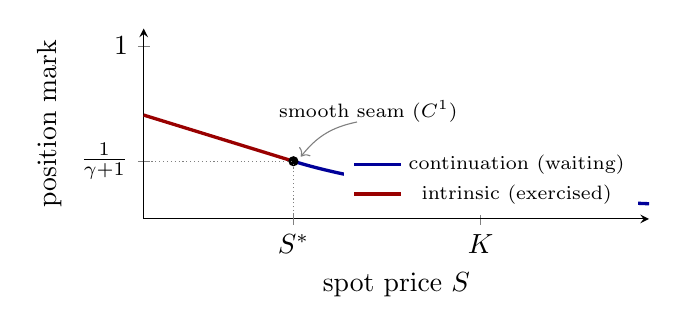
\begin{tikzpicture}
  \begin{axis}[
      width=8.0cm, height=4.0cm,
      xlabel={spot price $S$},
      ylabel={position mark},
      xmin=40, xmax=130, ymin=0, ymax=1.1,
      xtick={66.67,100}, xticklabels={$S^{\ast}$,$K$},
      ytick={0.333,1}, yticklabels={$\tfrac{1}{\gamma+1}$,$1$},
      axis lines=left, samples=160, clip=false,
      legend style={at={(0.98,0.02)},anchor=south east,font=\scriptsize,draw=none}]
    % continuation: c*s_N with s_N ~ S^{-gamma}; here gamma=2, normalized so value=1/3 at S*=66.67
    % continuation mark = (1/3)*(66.67/S)^2 for S >= S*
    \addplot[very thick,blue!60!black,domain=66.67:130] {0.3333*(66.67/x)^2};
    \addlegendentry{continuation (waiting)}
    % intrinsic on the bounded wing: 1 - S/K, for S <= S*
    \addplot[very thick,red!60!black,domain=40:66.67] {1 - x/100};
    \addlegendentry{intrinsic (exercised)}
    % seam marker
    \node[circle,fill=black,inner sep=1.3pt] at (axis cs:66.67,0.3333) {};
    \draw[densely dotted,gray] (axis cs:66.67,0) -- (axis cs:66.67,0.3333);
    \draw[densely dotted,gray] (axis cs:40,0.3333) -- (axis cs:66.67,0.3333);
    \node[font=\scriptsize] at (axis cs:80,0.62) {smooth seam ($C^1$)};
    \draw[->,gray] (axis cs:78,0.56) to[bend right=20] (axis cs:68,0.36);
  \end{axis}
\end{tikzpicture}
\caption{The three zones: out-of-the-money the mark follows the
\emph{continuation} curve; at the free boundary
$S^{\ast}=K\,g_{\mathrm{loc}}/(g_{\mathrm{loc}}+1)$ it joins the \emph{intrinsic}
payoff with matching value \emph{and} slope (a $C^{1}$ ``seam''). Drawn for $m=1$
($g_{\mathrm{loc}}=\gamma=2$), put leg, $K=\$100$, $S^{\ast}=\$66.67$, boundary
mark $\tfrac13$; for $m\neq1$ the seam moves to $g_{\mathrm{loc}}=m\gamma$. The
weld is \tfp{}\textsuperscript{L5,L6} (Appendix~\ref{app:lean}).}
\label{fig:seam}
\end{figure}

This is the paper's core construction, told from the holder's situation. A
put at strike $K$ splits spot into three zones (Figure~\ref{fig:seam}):
\begin{itemize}[leftmargin=1.6em,itemsep=1pt]
  \item \textbf{Out-of-the-money} ($S>K$): waiting; the mark follows the
    power law of Eq.~\eqref{eq:mark}.
  \item \textbf{In-the-money, still waiting} ($S^{\ast}<S\le K$): the
    \emph{same} power law continues through the strike---the strike is an
    ordinary interior point, nothing happens there.
  \item \textbf{Exercised} ($S\le S^{\ast}$): the mark \emph{is} the payoff
    line $1-S/K$, which joins the waiting curve tangentially at $S^{\ast}$.
\end{itemize}
The zone edge $S^{\ast}$ is an \emph{early-exercise free boundary}---a price
level \emph{solved for}, not fixed in advance---and it sits \emph{past} the
strike. In every zone the holder may close at the quoted mark, and the quoted
mark is never below the payoff\textsuperscript{L6}; calls mirror by
reflection.

\subsection{The construction}
While the holder waits, the position is worth its \emph{continuation value}
$c\cdot s_{N}$, where $s_{N}$ is the \emph{normalised strike coordinate} (the
strike in the curve's own scaled units, with value $\propto s_{N}\propto
S^{-\gamma}$) and $c$ fixes the overall level. Continuation \emph{pastes} onto the
exercised (intrinsic) payoff at the boundary under \emph{smooth pasting}---in
plain terms, the payoff line is \emph{tangent} to the waiting curve: the two
pieces agree in value and slope, no kink and no jump---two equations in the two
unknowns
$s_{N}^{\ast}$ and $c$. The solution is closed form:
\begin{equation}
  S^{\ast}=K\,\frac{g_{\mathrm{loc}}}{g_{\mathrm{loc}}+1}
         =K\,\frac{m\gamma}{m\gamma+1},
  \qquad
  \text{value fraction at the boundary}=\frac{1}{g_{\mathrm{loc}}+1},
  \label{eq:boundary}
\end{equation}
where $g_{\mathrm{loc}}=m\gamma$ is the lensed steepness. The boundary therefore
\emph{moves with the lens}, reducing to the base form
$S^{\ast}=K\gamma/(\gamma+1)$ only at $m=1$. The mark reaches its cap of $1$
only at \emph{full} exercise, not at the boundary (Figure~\ref{fig:seam}).
$S^{\ast}$ is a \emph{pricing} boundary, not a forced trigger---it is where a
rational holder would exercise and what the valuation assumes (settlement is
always holder-invoked, never automatic); on the bounded (spread) wing the
intrinsic $1-S/K$ caps at $1$, while a single uncapped option wing keeps
growing past $1$, as it should.

\subsection{A worked example (illustrative numbers)}
A fully worked put-leg example ($\gamma=2$, $K=\$100$, both $m=1$ and $m=3$
columns, each evaluated at \emph{its own} boundary) is tabulated in
Appendix~\ref{app:spec}. Every number in it is a \emph{mark}---the value of
one escrow unit read at that spot, as spot moves through the zones; nothing is
bought or sold in the table (a position of notional $q$ at spot $S$ is worth
$q\cdot\mathrm{mark}(S)$). At a glance: the boundary~\eqref{eq:boundary} sits at
$S^{\ast}=\$66.67$ for $m=1$ (boundary mark $1/3$) and rises to $\$85.71$ for
$m=3$ (mark $1/7$); the at-the-money marks are $0.148$ and $0.057$; below
$S^{\ast}$ the mark is simply intrinsic, $1-S/K$. The numbers are
\emph{illustrative}---chosen for arithmetic clarity, not calibrated to any
market and not a validation of anything.

\subsection{Why this is the American boundary, and the Merton tie}
The smooth-paste solution is not an arbitrary $C^{1}$ join: it is the
\emph{unique} solution of the value-and-slope system at any steepness $g$---hence
at $g_{\mathrm{loc}}=m\gamma$ (\tfp{} for generic $g$\textsuperscript{L4}). The pasted object of Figure~\ref{fig:seam}---the
power continuation welded onto the \emph{linear} exercised payoff in the dollar
frame---is \tfp{}\textsuperscript{L5,L6} as well: value and
slope match at $S^{\ast}$ for every $g>0$; the welded value function is
differentiable \emph{at} the seam, not merely arm-by-arm; the value-and-slope
system \emph{forces} $S^{\ast}=K\,g/(g+1)$ and the continuation level uniquely;
and the quoted value is never below the exercised payoff, strictly above it beyond
the boundary (put-wing pricing object as depicted; the call-wing value-and-slope
match is also checked). The boundary moreover \emph{maximises} the holder's value
over \emph{deterministic} exercise boundaries (a genuine variational result;
\tfp{}\textsuperscript{L7}). The identification with the \emph{stochastic}
optimal-stopping (Snell) boundary is \emph{named but not formalised}---a
placeholder obligation, not a discharged premise.

The boundary also ties to the classical perpetual-American (Merton) problem. Here
$r$ is the risk-free rate and $\sigma$ the underlying's return volatility ($r$
distinct from the rebase factor); $\gamma$ is the \emph{characteristic root} of
the underlying's log-price process. The roots are those of the
\emph{zero-net-carry} pricing ODE
$\tfrac{\sigma^{2}}{2}S^{2}V''(S)-rV(S)=0$ (no first-order term---that
absence \emph{is} the symmetric pairing: put root $-\gamma$, call root
$\gamma+1$, roots summing to $1$), and the product-of-roots (Vieta) relation
reads
\begin{equation}
  \gamma(\gamma+1)=2r/\sigma^{2},
  \qquad\text{in the regime }r>\sigma^{2},
  \label{eq:merton}
\end{equation}
the convention encoded by our Lean-verified Vieta sum/product
relations\textsuperscript{L8}. On the symmetric pairing $S^{\ast}$ is the Merton
boundary, with the Gaussian-slice limit \tfp{}\textsuperscript{L8}, and the
generalized-hyperbolic / Bessel-K distributional layer carried as
named hypotheses---exact on the log-normal (Gaussian) slice, conditional beyond it.
This distributional tie is stated at the base characteristic root $\gamma$ (the
unlensed $m=1$ slice); the lens then transports the \emph{engine} boundary to
$g_{\mathrm{loc}}=m\gamma$ by the same generic-$g$ uniqueness above.

\paragraph{How literally to read the Merton relation.}
As a literal calibration formula, \eqref{eq:merton} requires $r>\sigma^{2}$,
which fails at crypto-scale volatility; we use it as a \emph{theory anchor}
fixing the calibration \emph{direction} (higher volatility, lower $\gamma$,
fatter wings), with $\gamma$ and $m$ \emph{design parameters} chosen at
deployment---full discussion in Appendix~\ref{app:spec}.

\subsection{The seam, checked two ways}
At the boundary the value- and slope-match hold for every $g>0$, hence at
$g=m\gamma$---\tfp{} both in the curve's own coordinate\textsuperscript{L4}
and, for the welded linear seam of Figure~\ref{fig:seam}, in the dollar
frame\textsuperscript{L5}---and the out-of-the-money$\to$in-the-money
crossover lands at the dollar strike $K$ for all $\gamma$
(\tfp{}\textsuperscript{L4}). On the live engine, the shipped implementation
reproduces the worked-example table cell-for-cell to four decimal places, read off
the rendered interface---both $m$ columns, both arms, and the two boundary points
($\$66.67$ and $\$85.71$)---and the value-never-below-exercised-payoff property is
enforced as a hard engine gate. These are engine measurements, not Lean theorems.

% ===========================================================================
The mechanism's economic properties---the no-internal-arbitrage symmetry,
settlement, and the replication scope---are developed in full in
Appendix~\ref{app:properties}.

\section{Related work}\label{sec:related}
% ===========================================================================

The weighted constant-product invariant is from Balancer~\cite{balancer}, whose
Liquidity Bootstrapping Pools already use time-varying weights; our per-trade
update is a finer-grained, trade-driven analogue. CFMM pricing-oracle theory is
from Angeris et al.~\cite{angeris-cfmm,angeris-uniswap}, alongside Uniswap
v2/v3~\cite{uniswapv2,uniswapv3}. The translated-curve view of each trade is
Evans~\cite{evans2020}; the replication theory of
Angeris--Evans--Chitra~\cite{angeris-replicating}, instantiated in
RMM-01~\cite{rmm01}, chooses a trading function to replicate a target payoff---so
we do not claim the curve family as a contribution. InfinityPools~%
\cite{infinitypools} builds options-like exposure on concentrated liquidity, and
Panoptic~\cite{panoptic} is the closest oracle-free perpetual-options protocol; we
differ in pricing the whole continuum from one pool state and in the American free
boundary. QuantAMM's weight-dynamic AMM work~\cite{quantamm} is \emph{prior} (not
concurrent); we use the neutral ``per-trade weight-dynamic AMM'' descriptor. The
Lean-AMM line is anchored by Pusceddu--Bartoletti~\cite{pusceddu-bartoletti}; our
ledger extends it to the smooth-pasting boundary, the lens, and the
conditional-solvency stack, on Lean~4~\cite{lean4} and Mathlib~\cite{mathlib}. The
nearest analytic neighbour is loss-versus-rebalancing (LVR) of Milionis et
al.~\cite{lvr}: an LP position read as a continuum of short perpetual options is
the \emph{dual} of our sell-side construction, and the LVR framing covers our
small trader-borne \emph{round-trip residual} (open-then-reverse at the same ray;
quantitative treatment deferred).

\section{Limitations and open questions}\label{sec:limits}
Beyond the headline conditional solvency, the open surfaces are: exact replication
is per-wing $|\Gamma|\le1$ ($|\Gamma|>1$ a labelled approximation); single-pool
rigidity fixes the liquidity shape (level and skew, not smile curvature); the
Merton tie is exact only on the Gaussian slice, with the generalized-hyperbolic /
Bessel-K layer carried, not discharged; the Lean-verified layer is not
yet wired to the production engine (the bridge is an oracle, not a verified
extraction); the carved-perp settlement ledger, the funding equilibrium-drift
quantification and cash-transfer routing
(Section~\ref{sec:continuum} and Appendix~\ref{sec:frontier}), and the round-trip residual
are open---the reversed legs round-trip the pool exactly (Section~\ref{sec:exec});
the residual arises when an in-the-money leg settles to cash, so its opening swap
remains in the pool. Relatedly, all strikes read one shared curve, so each trade's
skew moves every other strike's mark: the core mechanic of
Section~\ref{sec:warp} read as an externality, unquantified here.

\paragraph{Incentive properties (informal).}
The construction carries its first-order incentives by design, each a stated law
rather than a theorem: funding is congestion pricing---the crowded side pays the
contrarian side in proportion to how far trades have skewed the curve from the
anchor (Section~\ref{sec:continuum}); the frozen transaction strike returns the
pool's reserves exactly on every leg reversed at close (an in-the-money leg
settles to cash instead), so no repricing profit is extractable from the pool's
reserves (Section~\ref{sec:exec}); the pool never holds premium, so liquidity
providers are exposed to the curve's skew, never to option payouts; and payouts
are borne by the side's own club with a hard stop at zero equity, so counterparty
risk is internalized per side, not socialized. None of this replaces an
equilibrium analysis; it states the mechanism's built-in pressure toward balance.

\paragraph{Mechanism design: open.}
Incentive compatibility of the funding schedule, strategic behaviour near the
exercise boundary $S^{\ast}$ and around the knob $m$, the participation
rationality of liquidity providers, and a welfare comparison against order-book
alternatives are explicitly open future work. They are where the formal spine
meets the market: the conditional-solvency hypotheses of
Appendix~\ref{sec:frontier} (a funding port that pays, one-way arbitrage, a ledger
that closes) are behavioural assumptions, and discharging them is a
mechanism-design task as much as a proof task.

\section{Conclusion}\label{sec:conclusion}
A single Balancer pool with one dynamic weight---run as a state-transition system
whose conservation law is applied at each trade's own point, and whose trades
\emph{skew} the curve---prices the entire out-of-the-money perpetual-option
continuum in closed form. Exercise is zoned by a closed-form
smooth-pasting boundary
$S^{\ast}=K\,m\gamma/(m\gamma+1)$ (put form; calls mirror) with a smooth
seam and no new parameters,
\tfp{}\textsuperscript{L4,L5,L6} and tied to the Merton problem,
plus a constant slope-multiplier lens $m$ acting as a vol-calibrated knob while
leaving the pool flow unchanged. On internal arbitrage we claim only what is
proved: a posited collar surplus vanishes iff the pool is symmetric. The honest
frontier is solvency: geometry is necessary (the no-floor
theorem\textsuperscript{L12}) but never sufficient, and solvency stays
\emph{conditional} on a funding port shown necessary but not discharged. Closing
that port hypothesis and wiring the Lean-verified layer to the
production engine are the principal future directions.

\paragraph{Drafting disclosure.}
Portions of this paper's prose were drafted and edited with the assistance of a
large language model, under the authors' direction; all mathematical content,
claims, numbers, and provenance labels were specified, reviewed, and verified by
the authors, with the Lean-verified results produced as described in
Appendix~\ref{sec:frontier}.

% ===========================================================================
\appendix
\section{Annex: properties---no internal arbitrage, settlement, replication}\label{app:properties}
\label{sec:props}
% ===========================================================================

\subsection{No internal arbitrage (the costless collar)}
The sharp statement concerns a \emph{costless collar}: a band whose sold and
bought legs are cash-neutral by construction. We do \emph{not} claim that no
composition of swaps yields a riskless edge---no formal result covers swap
compositions, and we make no such claim. What we establish is a symmetry.

\begin{proposition}[Collar surplus vanishes exactly at symmetry]\label{prop:collar}
The costless-collar capital-efficiency surplus is zero \emph{if and only if} the
pool is symmetric, $w=\tfrac12$. Under skew ($w\neq\tfrac12$) the surplus is
non-zero, with an explicit counterexample.
\end{proposition}

The biconditional is the substance---but the formalised surplus is a
\emph{posited} form, so this is a symmetry statement about that posited surplus,
best read as a \emph{conditional skeleton}, not an unconditional no-arbitrage
theorem over the production engine (\tfp{}\textsuperscript{L9}; the full scope
notes, the reflection reading of the symmetry, and the pool-motion caveat are in
Appendix~\ref{app:spec}).

\subsection{Settlement}\label{sec:settlement}
A position is opened as a \emph{band}---a composition of legs---against a
perpetual future the trader already holds, the \emph{origin perp}. At open the
band is minted against a carved slice of that perp, whose notional, equity, and
entry mark are frozen for the band's life, so settlement attribution cannot be
contaminated by unrelated perp activity. Settlement is therefore
\emph{perp-denominated}: a mark is a fraction of one escrow unit, so a leg of
notional $q$ is worth $q\cdot\mathrm{mark}$ \emph{perp units}, and dollars enter
only at the end: at close, the leg values are netted in perp units and the net
converts to cash at the carved slice's \emph{closing} equity---its dollar worth at
the reference price then---scaled by the payout law below. A band has two legs on
opposite wings; spot cannot be in-the-money on both at once, giving a clean
two-case settlement. The composite-ray closed form holds across the
out-of-the-money$\to$in-the-money boundary under the effective-strike substitution
(\tfp{}\textsuperscript{L10}). Settlement's auxiliary inputs are
pinned: cash conversion reads the external reference feed (the same feed that
drives rebases), and the financing strike is the dollar $K_{\mathrm{tx}}$ frozen
at open. Settlement \emph{values} are pool-mark reads---that is the construction's
point---and the in-/out-of-the-money regime test likewise reads the pool's marked
price; a leg crossing that boundary settles at a value continuous across it (the
closed form above), so there is no cliff-edge intrinsic grab at the boundary.
Trust in the reference feed is an explicit assumption.

\subsection{Replication scope: $|\Gamma|\le1$ exact, $|\Gamma|>1$ approximate}
Let $\Gamma$ be the \emph{hedge ratio}---a position's price-sensitivity to spot.
The construction replicates the target American payoff \emph{exactly} for
$|\Gamma|\le1$, a bound that is \emph{per wing}. The shipped instrument is a
vanilla \emph{opposite-wing band}---at most one leg in-the-money at a time---so
the active wing is always a single $|\Gamma|\le1$ leg and replication is exact for
the shipped product. The $|\Gamma|>1$ regime arises only outside that design
(same-wing stacking or single-leg leverage), where ``true American'' exercise and
``exact replication per wing'' cannot both hold; we scope it out of the product
but keep it \emph{disclosed} as a labelled approximation
(Appendix~\ref{sec:frontier}).

% ===========================================================================

\section{Annex: mechanism specifications and worked example}\label{app:spec}

\subsection{The rebase, in full}
A rebase fires on each oracle update (whenever the external reference price
moves), with factor $r=S_{\mathrm{new}}/S_{\mathrm{old}}$. It is one rescaling
of the pricing frame:
\[
  x\to r\,x,\qquad \alpha\to r\,\alpha,\qquad
  y,\ \beta,\ w\ \text{invariant},\qquad
  \theta\to\theta/r\ \text{(each strike ray)},\qquad k\to r^{w}k .
\]
In simple terms: the curve and every strike ray are re-zoomed \emph{together},
so the pool's centre tracks the outside price. Three implications, each
load-bearing: (i)~a rebase is a \emph{gauge move}---a change of coordinates,
not a trade: every normalized quantity (moneyness, marks, position values) is
invariant, so no position gains or loses from a rebase; (ii)~trades and rebases
\emph{commute} (\tfp{}\textsuperscript{L2}), so the pricing
frame is well defined no matter how trades interleave with oracle updates; and
(iii)~by re-centering the frame on every oracle move it bounds how fast drift
can accumulate into the funding deviation of Section~\ref{sec:continuum}.

\subsection{The funding rate law (shipped form)}
Per position of notional $N$ at strike ray $\theta$, per unit time,
\[
  \text{funding rate}
  \;=\;
  \kappa\cdot(\pm g_{\mathrm{loc}})\cdot N\cdot
  \mathrm{mark}(\theta)\cdot\frac{\Sigma-1}{\Sigma},
  \qquad
  \Sigma=\frac{\text{pool-marked price}}{\text{reference price}},
\]
with $\kappa$ a rate constant, the sign $+$ for calls and $-$ for puts (this
sign pairing is what makes the crowded side pay the contrarian side),
$g_{\mathrm{loc}}=m\gamma$ the lensed steepness of Section~\ref{sec:lens},
$\mathrm{mark}(\theta)$ the position's own mark, and $\Sigma$ the deviation
ratio of the live (skewed) curve from the anchor. On-anchor ($\Sigma=1$) the
rate is exactly zero. This is the shipped design law (a specification, not a
Lean-verified result); the cash transfer it meters remains
implementation-level (Section~\ref{sec:continuum}).

\subsection{Worked example (illustrative numbers), in full}
Every cell below is a \emph{mark}: the value of \emph{one escrow unit} read
at that spot---the read as spot moves through the zones of
Section~\ref{sec:american}. No transaction occurs in this table; a position
of notional $q$ is worth $q\cdot\mathrm{mark}$ at each spot. The values are
\emph{illustrative}---chosen for arithmetic clarity, not calibrated
to any market and not a validation of anything. Take a put leg with $\gamma=2$,
$K=\$100$, $m=1$ ($g_{\mathrm{loc}}=2$). The boundary~\eqref{eq:boundary} sits at
$S^{\ast}=100\cdot\tfrac23=\$66.67$, below the strike, with mark
$1/(g_{\mathrm{loc}}+1)=1/3$ there. Steepening to $m=3$ ($g_{\mathrm{loc}}=6$)
\emph{moves} the boundary---$C^{1}$ smooth-pasting forces the boundary and the
continuation arm to share the same exponent $g_{\mathrm{loc}}$---rising to
$S^{\ast}=100\cdot\tfrac{6}{7}=\$85.71$ with boundary mark
$1/(g_{\mathrm{loc}}+1)=1/7\approx0.143$; below $S^{\ast}$ the leg is simply
intrinsic, $1-S/K$. The continuation mark also decays faster, via the wing power
law $\mathrm{value}\propto S^{-g_{\mathrm{loc}}}$. Each column below is evaluated
at \emph{its own} boundary:
\begin{center}
\begin{tabular}{lcc}
\toprule
spot $S$ & mark, $m=1$ ($g_{\mathrm{loc}}=2$) & mark, $m=3$ ($g_{\mathrm{loc}}=6$) \\
\midrule
at $S^{\ast}$ & $0.333$ (at $\$66.67$) & $0.143$ (at $\$85.71$) \\
$\$80$  & $0.231$ & $0.200$ \\
$\$90$  & $0.183$ & $0.107$ \\
$\$100=K$ & $0.148$ & $0.057$ \\
$\$120$ & $0.103$ & $0.019$ \\
\bottomrule
\end{tabular}
\end{center}
Below $S^{\ast}$ the mark is intrinsic ($1-S/K$): at $m=3$, $\$80<\$85.71$, so its
mark is $1-80/100=0.200$. The table traces~\eqref{eq:boundary} and the wing power
law; it makes no empirical or market-calibration claim.

\subsection{The costless collar: scope notes}
The biconditional is the substance. The formalised surplus is a \emph{posited}
form proportional to anchor asymmetry, so the result is a symmetry statement about
that posited surplus, not a mechanism-level no-arbitrage theorem over swap
compositions; we carry it as a named definition with the skew sign exhibited
(\tfp{}\textsuperscript{L9}). A companion result casts the symmetry as a
reflection---the put at coordinate $s$ is the call reflected through the
at-the-money ray ($s\mapsto\theta^{2}/s$)---so no-arbitrage \emph{is} the curve's
symmetry (\tfp{}\textsuperscript{L9}). The reflection arrow is a proved identity,
but the link from the spec mark to the live engine's instrument is a residual
modeling premise, so this is best read as a \emph{conditional skeleton}, not an
unconditional no-arbitrage theorem over the production engine.

A costless collar is not free of \emph{pool motion}---its two legs move $w$---but
the trader pays for that displacement at fair, sequenced prices (a swap's proceeds
are the path integral of the marginal price): no free cash. Zero skew removes the
\emph{free} edge, not the \emph{worth} of the protection.

\subsection{The Merton relation: how literally to read it}
As a literal calibration formula, \eqref{eq:merton} lives in the regime
$r>\sigma^{2}$, which fails at crypto-scale volatility ($\sigma\approx80\%$ would
demand $r>64\%$). We use it as a \emph{theory anchor}: it fixes the
\emph{direction} of calibration---higher volatility, lower $\gamma$, fatter wings
(Section~\ref{sec:idea})---and is exact on the Gaussian slice, but $\gamma$ and
$m$ are \emph{design parameters} chosen at deployment, not quantities implied
from market $r$ and $\sigma$ through the formula.

% ===========================================================================
% NOTE: The notation table and the formal-artifact map live in the on-request
% supplement (not attached). Every symbol is glossed in-body at first use.
% ===========================================================================

\section{Annex: index of Lean-verified results}\label{app:lean}
Each superscript L$n$ in the body refers to one row below. All rows carry the
same provenance: verified in Lean~4 by Harmonic's Aristotle prover, compiled
server-side, artifact-audited, not re-run locally
(Appendix~\ref{sec:frontier}); the actual Lean proofs are available on
request. The rows are statements about the specification-level objects of the
formal development, not about the production engine's code; the engine bridge
is measured, not extracted (Appendix~\ref{sec:frontier}).
\begin{center}
\begin{tabularx}{\textwidth}{@{}l X l@{}}
\toprule
 & what is verified in Lean & Lean identifiers \\
\midrule
L1 & The pool invariant and the trade law of Eq.~\eqref{eq:tradeupdate}:
     conservation applied at the trade's own point, with the weight update.
     (The off-the-money trade-point existence/uniqueness lemmas report complete
     at the prover but are not folded to this bar and are not counted.)
     & \texttt{invariant}, \texttt{trade\_dx} \\
L2 & Trades and rebases commute; the pricing frame is order-independent.
     & \texttt{trade\_rebase\_commute} \\
L3 & The lens sets the option-value steepness to $m\gamma$ uniformly at every
     strike and leaves the pool's trade dynamics unchanged.
     & \texttt{gLoc\_*}, pool-unchanged facts \\
L4 & Smooth pasting in the curve's own coordinate: value and slope match at
     every steepness $g>0$; boundary and level are forced (unique); the
     OTM$\to$ITM crossover lands at the dollar strike $K$.
     & \texttt{valueMatch\_g}, \texttt{slopeMatch\_g},
       \texttt{Sstar\_A\_forced}, \texttt{crossover\_sNorm\_at\_K} \\
L5 & The linear seam of Figure~\ref{fig:seam}, dollar frame: the power
     continuation meets the linear exercised payoff with matching value and
     slope; the welded value function is differentiable at the boundary (no
     kink); the value-and-slope system forces $S^{\ast}=Kg/(g+1)$ and the
     continuation level uniquely (put wing; call-wing value/slope match also
     checked). & \texttt{paste\_value\_lin}, \texttt{paste\_slope\_lin},
       \texttt{Vp\_hasDerivAt\_seam}, \texttt{paste\_unique} \\
L6 & American consistency: the quoted value is never below the exercised
     payoff, strictly above it beyond the boundary (put-wing pricing object).
     & \texttt{value\_ge\_intrinsic},
       \texttt{value\_gt\_intrinsic\_beyond\_seam} \\
L7 & The boundary maximises holder value over \emph{deterministic} exercise
     policies (the stochastic Snell identification is \emph{not} formalised).
     & \texttt{opt\_boundary\_is\_max\_A} \\
L8 & The Merton tie: the symmetric-pairing Vieta relations behind
     $\gamma(\gamma+1)=2r/\sigma^{2}$, the boundary as the Merton boundary on
     that pairing, and the Gaussian-slice limit.
     & \texttt{merton\_vieta\_sum/prod},
       \texttt{Sstar\_is\_merton\_boundary}, \texttt{gaussian\_limit\_quadratic} \\
L9 & Collar symmetry: the posited costless-collar surplus is zero iff
     $w=\tfrac12$, with a skew counterexample; the put--call reflection
     identity through the at-the-money ray.
     & \texttt{collarSurplus\_zero\_iff\_half}, \texttt{reflection\_arrow} \\
L10 & Settlement: the composite-ray closed form holds across the OTM$\to$ITM
     boundary under the effective-strike substitution.
     & \texttt{compositeRay\_ITM\_substitution} \\
L11 & The conditional-solvency stack: pool-value concavity propagates
     curve$\to$storage by types; \emph{given} the B1/B3/B4 hypotheses,
     passivity and solvency; proven instances: the equal-weight
     constant-product pool and an exponential pool.
     & solvency stack, \texttt{cpmm}/\texttt{expPool} instances \\
L12 & \texttt{reserves\_have\_no\_floor}: with a convex obligation, reserve
     value is unbounded below---the solvency floor cannot come from reserves
     (``convexity must be funded'' as a theorem).
     & \texttt{reserves\_have\_no\_floor} \\
L13 & The internal (passivity) half of the single-object direction: the system
     is passive because its geometry is positive semidefinite.
     & \texttt{internal\_passivity} \\
\bottomrule
\end{tabularx}
\end{center}
Two representative statements from the compiled Lean source (ASCII-set: `R'
for the reals, `<=' for $\le$; put wing; \texttt{sStarP g K = K*g/(g+1)},
\texttt{contP} the power continuation, \texttt{intrP} the linear intrinsic,
\texttt{Vp} the pasted value):
\begin{verbatim}
theorem paste_value_lin (g K : R) (hg : 0 < g) (hK : 0 < K) :
    contP g K (sStarP g K) = intrP g K (sStarP g K)        -- L5

theorem value_ge_intrinsic (g K S : R) (hg : 0 < g)
    (hK : 0 < K) (hS : 0 < S) :
    max (1 - S / K) 0 <= Vp g K S                           -- L6
\end{verbatim}
Full formal statements, the complete Lean proofs, and a complete working
implementation of the mechanism (a self-contained simulator) are available
from the authors on request.

% ===========================================================================
\section{Annex: formal verification and the open frontier}\label{sec:frontier}
% ===========================================================================

\subsection{Provenance: verified in Lean by Harmonic's Aristotle}
Every result marked \emph{verified in Lean} is indexed by a superscript
L1--L13, one row each in Appendix~\ref{app:lean}, with its Lean identifiers.
Each was proved and compiled in Lean~4.28.0 / Mathlib~v4.28.0 by Harmonic's
\emph{Aristotle} prover (server-side), and the returned artifacts passed our
audit: forbidden-token scan, \texttt{\#print axioms} restricted to
$\{\texttt{propext},\texttt{Classical.choice},\texttt{Quot.sound}\}$, an
unscoped-module diff, and a hand re-derivation of each statement. The compiled
proofs were not re-run against a local kernel; the label states the provenance
as it is. We distinguish \emph{grounded} results (no load-bearing carried
hypothesis) from \emph{carried} results (conditional on named, undischarged
structure-field hypotheses---never on \texttt{axiom}s). \textbf{The actual
Lean proofs are available on request} (anonymized artifact repository), and so
is a \textbf{complete working implementation}---a self-contained simulator of
the full mechanism; two
representative statements are reproduced verbatim in
Appendix~\ref{app:lean}.

\subsection{Solvency is conditional---the headline open item}
The construction's solvency guarantee is \emph{conditional}. A separate prover
line formalises the curve\,$\to$\,value\,$\to$\,storage interface as a typed stack
and proves (\tfp{}\textsuperscript{L11}): pool value is concave in price
for any valid curve and this propagates into stored equity by types; and the
headline \texttt{reserves\_have\_no\_floor}\textsuperscript{L12}---with a convex
obligation, reserve value is unbounded below, so \emph{the solvency floor cannot
come from reserves} (``convexity must be funded'' as a theorem). It then proves:
\emph{given} a port that covers the concave deficit, the pool is passive and
solvent for all time with no free lunch.

That ``given'' is the whole point. The hypotheses---B1 (a funding port covers the
floor), B3 (arbitrage is one-way), and B4 (the settlement ledger closes)---are
carried as \emph{structure fields}, not discharged facts. The stack proves
``\emph{if} the ledger closes, arbitrage is one-way, and the port covers the
floor, \emph{then} passivity and solvency''; it does \emph{not} prove the port
pays in the real world. Geometry is shown \emph{necessary} (the no-floor
theorem\textsuperscript{L12}) but never \emph{sufficient}. These are
\emph{assumptions, not claims}; the reader should not mistake conditional solvency
for an unconditional result. The proven instances are the equal-weight
constant-product pool and an exponential pool\textsuperscript{L11}; the lensed
American construction of Sections~\ref{sec:lens}--\ref{sec:american} is not yet an
instance of the stack, and the typed contracts are \emph{not} yet wired to the
production engine's numeric formulas---that instantiation is the next body of
work.

\subsection{The whole exchange as a single object (research direction)}
A partial result unifies the entire exchange---storage, flow, funding port,
settlement, dollar pipe---as one passive object whose solvency reads as
passivity-under-admissible-inputs. The \emph{internal} half is
\tfp{}\textsuperscript{L13}: the system is passive because its geometry is
positive-semidefinite. The \emph{external}/solvency half stays \emph{open},
keeping the coverage premise undischarged and honoring the no-floor
theorem\textsuperscript{L12}; we present the single object as a conjecture /
research direction, not a finished proven artifact.

% ===========================================================================

% ===========================================================================
\begin{thebibliography}{99}

% [one never-cited bibitem removed for double-blind.]

\bibitem{uniswapv2}
H.~Adams, N.~Zinsmeister, and D.~Robinson. \emph{Uniswap v2 Core.} 2020.

\bibitem{uniswapv3}
H.~Adams, N.~Zinsmeister, M.~Salem, R.~Keefer, and D.~Robinson.
\emph{Uniswap v3 Core.} 2021.

\bibitem{angeris-cfmm}
G.~Angeris and T.~Chitra. Improved Price Oracles: Constant Function Market Makers.
In \emph{Proc. 2nd ACM Conf. on Advances in Financial Technologies (AFT '20)}, 2020.

\bibitem{angeris-uniswap}
G.~Angeris, H.-T.~Kao, R.~Chiang, C.~Noyes, and T.~Chitra.
An Analysis of Uniswap Markets. \emph{Cryptoeconomic Systems}, 2019.

\bibitem{balancer}
F.~Martinelli and N.~Mushegian.
\emph{Balancer: A Non-Custodial Portfolio Manager, Liquidity Provider, and Price
Sensor.} 2019.

\bibitem{panoptic}
G.~Lambert and J.~Kristensen.
\emph{Panoptic: a perpetual, oracle-free options protocol.} arXiv:2204.14232, 2022.

\bibitem{evans2020}
A.~Evans. \emph{Liquidity Provider Returns in Geometric Mean Markets.}
arXiv:2006.08806, 2020.

\bibitem{angeris-replicating}
G.~Angeris, A.~Evans, and T.~Chitra. \emph{Replicating Market Makers.}
arXiv:2103.14769, 2021.

\bibitem{rmm01}
Primitive Finance. \emph{Replicating Market Makers (RMM-01).}
Protocol whitepaper, 2021.

\bibitem{infinitypools}
InfinityPools. \emph{InfinityPools: leverage and options on concentrated
liquidity.} Protocol documentation, 2023.

\bibitem{quantamm}
M.~Willetts and C.~Harrington. \emph{Optimal Rebalancing in Dynamic AMMs.}
arXiv:2403.18737, 2024.

\bibitem{pusceddu-bartoletti}
N.~Pusceddu and M.~Bartoletti.
\emph{A formal model of Automated Market Makers in the Lean theorem prover.}
In \emph{6th Workshop on Formal Methods for Blockchains (FMBC 2024)}.
arXiv:2402.06064, 2024.

\bibitem{lvr}
J.~Milionis, C.~C.~Moallemi, T.~Roughgarden, and A.~L.~Zhang.
\emph{Automated Market Making and Loss-Versus-Rebalancing.}
arXiv:2208.06046, 2022.

\bibitem{lean4}
L.~de Moura and S.~Ullrich.
The Lean 4 Theorem Prover and Programming Language.
In \emph{Automated Deduction -- CADE 28}, 2021.

\bibitem{mathlib}
The mathlib Community. The Lean Mathematical Library.
In \emph{Proc. 9th ACM SIGPLAN Int. Conf. on Certified Programs and Proofs
(CPP '20)}, 2020.

\end{thebibliography}

\end{document}
